\documentclass[12pt]{scrartcl}

% packages
\usepackage[
    a4paper, total={18cm, 26cm},
    left=0.75in,
    right=0.75in,
    top=0.75in,
    bottom=0.50in,
    footskip=15pt
]{geometry}
\usepackage{lastpage}
\usepackage{graphicx} % \includegraphics
\usepackage{amsmath} % math
\usepackage{fancyhdr} % header and footer
\usepackage[portuguese]{babel}
\usepackage{tabularx}
\usepackage{listings}

% configs
\setlength{\parindent}{0pt}

% comandos
\renewcommand{\familydefault}{\sfdefault}
\newcommand{\un}[1]{\;\textrm{#1}}
\newcommand{\logo}{\quad \Rightarrow \quad}
\newcommand{\fase}[1]{\ensuremath{\phase{{#1}^{\circ}}}}
\newcommand{\code}[1]{\texttt{#1}}

\graphicspath{ {./images/} }

\begin{document}

\lstset{frame=none,
  language=R,
  aboveskip=3mm,
  belowskip=3mm,
  showstringspaces=false,
  columns=flexible,
  basicstyle={\small\ttfamily},
  numbers=none,
  breaklines=true,
  breakatwhitespace=true,
  tabsize=4
}


\numberwithin{figure}{section}
\numberwithin{equation}{section}
\numberwithin{table}{section}

\pagestyle{fancy}

\fancyhead{}
\fancyhead[L]{Avaliação 2 - Algoritmo Coeficiente Convectivo}
\fancyhead[R]{EMA255 - Termodinâmica Computacional}
\fancyfoot{}
\fancyfoot[R]{Pág. \thepage \; / \pageref{LastPage}}

\begin{center}
    Aluno: Raphael Henrique Braga Leivas \\
    Matrícula: 2020028101 \\
    Professor Responsável: Márcio Ziviani \\[20pt]

    Código fonte LaTeX desse arquivo pode ser visto em meu GitHub pessoal: https://github.com/RaphaelLeivas/latex/tree/main/TermoComp
\end{center}

\hrule

\section{Problema}

Precisamos criar um algoritmo para determinar a temperatura de equilíbrio da superfície
da parede esquerda $T_e$ de uma placa vertical. Temos as seguintes informações dadas:

\begin{itemize}
    \item Condutividade térmica: $k=2,5 \un{W/m$^2$K}$
    \item Comprimento: $W=5,0 \un{m}$
    \item Altura: $H=2,0 \un{m}$
    \item Espessura: $L=0,25 \un{m}$
    \item Velocidade do ar ambiente na face da parede: $u_{\infty}=3 \un{m/s}$
    \item Temperatura do ar ambiente na face da parede: $T_{\infty}=300 \un{K}$
    \item Fluxo de calor prescrito sobre a parede esquerda: $q_{p}^{''}=750 \un{W/m$^2$}$
    \item Temperatura da parede direita: $T_d=350 \un{K}$
\end{itemize}

\section{Solução}

De posse dessas informações, fazemos um desenho esquemático do problema, exibido na
Figura \ref{fig:problemaParede}.

\begin{figure}[h!]
    \caption{Diagrama do problema posto, com superfície de controle destacada.}
    \label{fig:problemaParede}
    \centering
    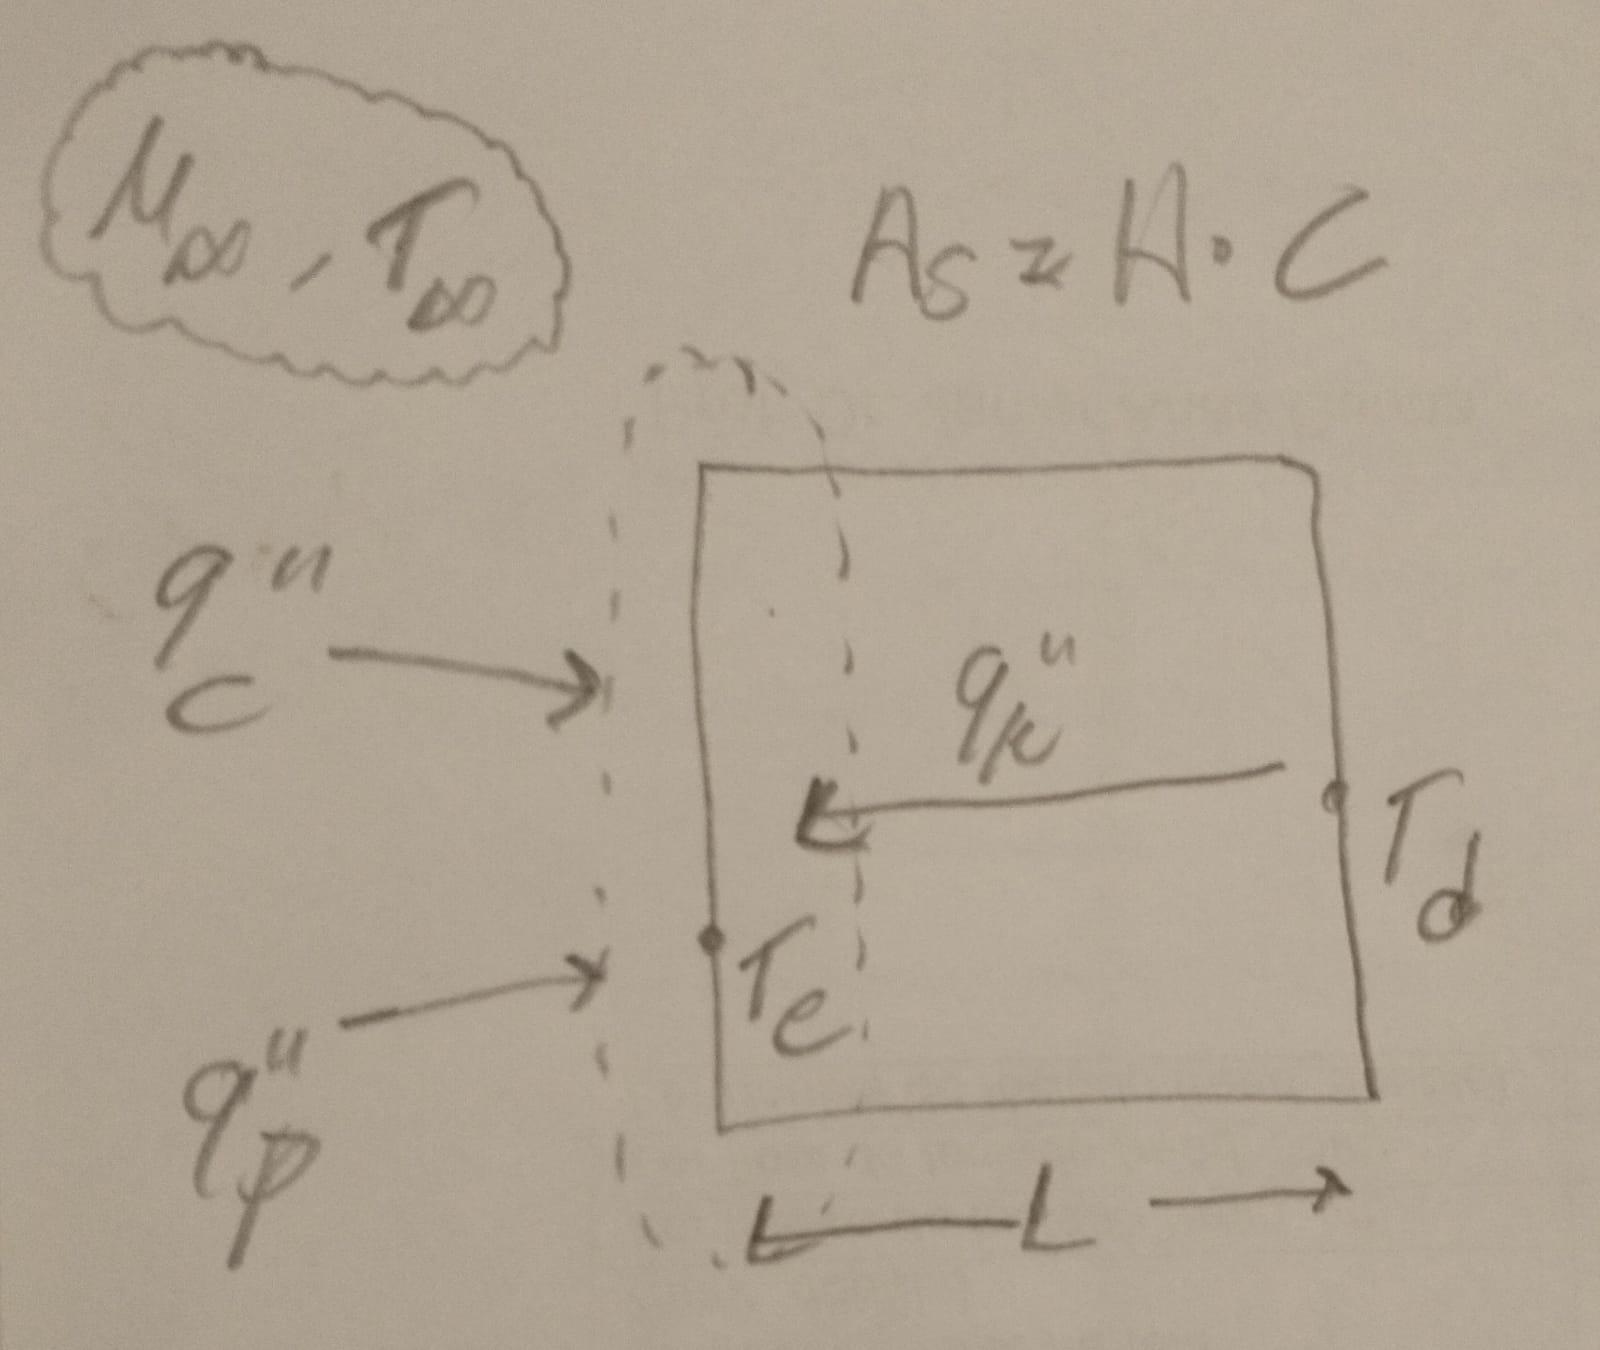
\includegraphics[scale=0.18]{esquematico.jpeg}
    \par{Fonte: elaboração própria.}
\end{figure}

Como mostra a Figura \ref{fig:problemaParede}, traçamos uma superfície de controle na
parede esquerda. Aplicando a primeira lei da termodinâmica sobre essa superfície, temos

\begin{equation}\label{eq:primeiraLei}
    \overset{\cdot}{E}_{in} + \overset{\cdot}{E}_{g} - \overset{\cdot}{E}_{out} = \overset{\cdot}{E}_{st}
\end{equation}

Como temos uma superfície de controle, não há energia armazenada e nem energia gerada. Além disso, no modelo
da Figura \ref*{fig:problemaParede}, repare que todos os fluxos de calor estão entrando na superfície, de tal
maneira que $\overset{\cdot}{E}_{out} = 0$. Assim, \eqref{eq:primeiraLei} se reduz a

\begin{equation}\label{eq:primeiraLeiReduzida}
    \overset{\cdot}{E}_{in} = 0
\end{equation}

Expandindo o termo $\overset{\cdot}{E}_{in}$,

\[ q_{p}^{''} + q_{c}^{''} + q_{k}^{''} = 0 \]

\[ q_{p}^{''} + h_c\left(T_{\infty}-T_e\right) + \frac{k}{L}\left(T_d-T_e\right) = 0 \]

Isolando o coeficiente convectivo $h_c$, temos

\[ h_c\left(T_{\infty}-T_e\right) = - q_{p}^{''} - \frac{k}{L}\left(T_d-T_e\right)\]

\begin{equation}\label{eq:hc}
    h_c = - \frac{q_{p}^{''} + \frac{k}{L}\left(T_d-T_e\right)}{T_{\infty}-T_e}
\end{equation}

Como a velocidade do ar ambiente na face da parede é $u_{\infty}=3 \un{m/s}$, temos que isso equivale a
$10,8 \un{km/h}$. Para ter uma noção do quão rápido essa velocidade é, usamos a Tabela \ref*{tab:winds}.

\begin{table}[h!]
    \caption{Relação entre a velocidade do vento e seu efeito.}
    \label{tab:winds}
    \begin{center}
        \begin{tabularx}{0.75\textwidth} {
                | >{\centering\arraybackslash}X
                | >{\centering\arraybackslash}X
                | >{\centering\arraybackslash}X |}
            \hline
            Nº de Beaufort & Descrição  & Velocidade do vento (km/h) \\
            \hline
            0              & Calmo      & $< 1.6$                    \\
            \hline
            1              & Ar leve      & $1.6$ a $4.8$              \\
            \hline
            2              & Brisa leve & $6.4$ a $11.2$             \\
            \hline
        \end{tabularx}
    \par{Fonte: Traduzido de National Oceanic and Atmospheric Administation (NOAA). Disponível em: https://www.weather.gov/pqr/wind.}
    \end{center}
\end{table}

Assim, segundo a Tabela \ref*{tab:winds}, temos que $u_{\infty} = 10,8 \un{km/h}$ equivale a apenas uma brisa leve, e portanto
podemos considerar a convecção como natural. 
\underline{Nota}: tentamos considerar a convecção como forçada, mas encontramos erros, conforme elaborado na seção \ref{discussion}. \\

Uma vez feita a análise inicial do problema, agora criamos um código em linguagem R para 
calcular iterativamente a temperatura da face esquerda até ela convergir para 
para a temperatura de equilíbrio. O primeiro passo é adicionar os dados do problema no código  

\begin{lstlisting}
    # dados do problema
    k <- 2.5
    W <- 5
    H <- 2
    L <- 0.25
    u_inf <- 3
    T_inf <- 300
    q_pres <- 750
    T_d <- 350
\end{lstlisting}

Em seguida, definimos a tabela com as propriedades termofísicas do ar conforme o livro
do Incropera. A primeira coluna da variável \code{Properties\char`_Table} representa a temperatura do fluido, e as demais colunas representação
respectivamente as propriedades termofísicas de massa específica $\rho$, viscosidade dinâmica $\mu$, viscosidade
cinética $v$, condutividade térmica do fluido $k_f$ e número de Prandtl $Pr$.

\begin{lstlisting}
    Properties_Table = matrix(
        c(
          100, 3.5562, 71.1 * 10^-7, 2.00 * 10^-6, 9.34 * 10^-3, 0.786,
          150, 2.3364, 103.4 * 10^-7, 4.426 * 10^-6, 13.8 * 10^-3, 0.758,
          200, 1.7458, 132.5 * 10^-7, 7.590 * 10^-6, 18.1 * 10^-3, 0.737,
          250, 1.3947, 159.6 * 10^-7, 11.44 * 10^-6, 22.3 * 10^-3, 0.720,
          300, 1.1614, 184.6 * 10^-7, 15.89 * 10^-6, 26.3 * 10^-3, 0.707,
          350, 0.9950, 208.2 * 10^-7, 20.92 * 10^-6, 30.0 * 10^-3, 0.700,
          400, 0.8711, 230.1 * 10^-7, 26.41 * 10^-6, 33.8 * 10^-3, 0.690,
          450, 0.7740, 250.7 * 10^-7, 32.39 * 10^-6, 37.3 * 10^-3, 0.686,
          500, 0.6964, 270.1 * 10^-7, 38.79 * 10^-6, 40.7 * 10^-3, 0.684,
          550, 0.6329, 288.4 * 10^-7, 45.57 * 10^-6, 43.9 * 10^-3, 0.683,
          600, 0.5804, 305.8 * 10^-7, 52.69 * 10^-6, 46.9 * 10^-3, 0.685
        ),
        ncol = 6,
        byrow = TRUE
    )
      
    colnames(Properties_Table) <- c('Tf', 'rho', 'mu', 'v', 'kf', 'Pr')
    rownames(Properties_Table) <- seq(1, nrow(Properties_Table), 1)
    Properties_Table <- as.table(Properties_Table)
\end{lstlisting}

Agora definimos uma variável \code{max\char`_iterations} que limita o número máximo de
iterações para que $T_e$ converja, a fim de evitar loops infinitos em tempo de compilação.
Além disso, definimos o valor inicial ("chute") para $T_e$, e o adicionamos em uma lista
que salva os valores calculados de $T_e$ em cada iteração. Consideramos o valor inicial de
$T_e$ como a temperatura ambiente $T_e = 25 \un{°C} = 298 \un{K}$.

\begin{lstlisting}
    max_iterations <- 100
    T_e_calculated <- 298 # chute inicial: Te = 298K (ambiente)
    T_e_list <- c(T_e_calculated)
\end{lstlisting}

Agora definimos um loop \code{for}, em que cada iteração se calcula um valor de $T_e$ até que ele converja.

\begin{lstlisting}
    for (i in 1:max_iterations) {
    
    }
\end{lstlisting}

Dentro de cada iteração do loop, inicializamos uma variável $T_f$, que é a temperatura do fluido em 
que olharemos na tabela, definida por  

\begin{equation}\label{eq:tf}
    T_f = \frac{T_e + T_{\infty}}{2}
\end{equation}

No código, \eqref{eq:tf} é executada por

\begin{lstlisting}
    Tf <- (T_e_calculated + T_inf) / 2
\end{lstlisting}

O próximo passo é percorrer a tabela das propriedades termofísicas, identificando
as temperaturas $T_{f_{min}}$ e $T_{f_{max}}$ entre as quais a temperatura $T_f$ se encontra, isto é, 
a faixa $T_{f_{min}} \leq T_f \leq T_{f_{max}}$.

\begin{lstlisting}
    # iniciais
    Tf_min <- Properties_Table[1, 'Tf']
    Tf_min_index <- 1
    Tf_max <- Properties_Table[nrow(Properties_Table), 'Tf']
    Tf_max_index <- nrow(Properties_Table)
    
    # procura na tabela alguem com esse valor de Tf
    for (j in 1:nrow(Properties_Table)) {
      if (Properties_Table[j, 'Tf'] <= Tf) {
        Tf_min <- Properties_Table[j, 'Tf']
        Tf_min_index <- j
      }
      
      if (Properties_Table[j, 'Tf'] > Tf) {
        Tf_max <- Properties_Table[j, 'Tf']
        Tf_max_index <- j
        break
      }
    }
\end{lstlisting}

Isso deve ser feito pois $T_f$ pode não coincidir exatamente com os valores tabelados.
Assim, usamos a variável \code{interpolation\char`_ratio} para realizar a interpolação dos valores  
das propriedades, dependendo do quão próximo $T_f$ está de $T_{f_{min}}$ ou $T_{f_{max}}$.

\begin{lstlisting}
    interpolation_ratio <- (Tf - Tf_min) / (Tf_max - Tf_min)
\end{lstlisting}

Com a razão de interpolação, calculamos as propriedades termofísicas necessárias através de interpolação 
com os dados da tabela.

\begin{lstlisting}
    rho_min <- Properties_Table[Tf_min_index, 'rho']
    rho_max <- Properties_Table[Tf_max_index, 'rho']
    rho <- rho_min + (rho_max - rho_min) * interpolation_ratio
    
    mu_min <- Properties_Table[Tf_min_index, 'mu']
    mu_max <- Properties_Table[Tf_max_index, 'mu']
    mu <- mu_min + (mu_max - mu_min) * interpolation_ratio
    
    v_min <- Properties_Table[Tf_min_index, 'v']
    v_max <- Properties_Table[Tf_max_index, 'v']
    v <- v_min + (v_max - v_min) * interpolation_ratio
    
    kf_min <- Properties_Table[Tf_min_index, 'kf']
    kf_max <- Properties_Table[Tf_max_index, 'kf']
    kf <- kf_min + (kf_max - kf_min) * interpolation_ratio
    
    Pr_min <- Properties_Table[Tf_min_index, 'Pr']
    Pr_max <- Properties_Table[Tf_max_index, 'Pr']
    Pr <- Pr_min + (Pr_max - Pr_min) * interpolation_ratio
\end{lstlisting}

Com as propriedades termofísicas calculadas, agora calculamos os coeficientes
adimensionais

\begin{lstlisting}
    Re_critical <- 50000
    Re <- u_inf * L * rho / mu
    Nu <- 0.0
    Gr <- 9.81 * (1/Tf) * (abs(T_e_calculated - T_inf) * L^3) / (v^2)
    Ra <- Gr * Pr

    Nu <- (0.825 + (0.387 * Ra^(1/6)) / (1 + (0.492/Pr)^(9/16))^(8/27))^2
\end{lstlisting}

Note que, para o cálculo do Número de Nusselt, usamos a expressão \eqref{eq:Nu}, que 
é a mesma para escoamentos laminar e turbulento em uma placa plana vertical.

\begin{equation}\label{eq:Nu}
    Nu = \left\{ 0,825 + \frac{0,387Ra^{1/6}}{\left[1 + \left(0,492 / Pr\right)^{9/16}\right]^{8/27}} \right\}^2
\end{equation}

Encontramos o coeficiente convectivo $h_c$ através de 

\begin{equation}\label{eq:hc_Nu}
    h_c = \frac{Nu \cdot K_f}{L}
\end{equation}

No código, 

\begin{lstlisting}
    hc <- Nu * kf / L
\end{lstlisting}

Com $h_c$ calculado, encontramos a temperatura da face esquerda
através da expressão \eqref{eq:hc}, isolando $T_e$, obtendo

\[ h_cT_{\infty} - h_cT_e = - q_{p}^{''} - \frac{k}{L}T_d + \frac{k}{L}T_e \]

\[  - T_e\left(h_c + \frac{k}{L}\right) = - h_cT_{\infty} - q_{p}^{''} - \frac{k}{L}T_d \]

\begin{equation}\label{eq:te}
    T_e = \frac{h_cT_{\infty} + q_{p}^{''} + \frac{k}{L}T_d}{h_c + \frac{k}{L}}
\end{equation}

No código, calculamos $T_e$ através de \eqref{eq:te} e o inserimos na lista de $T_e$ calculados

\begin{lstlisting}
    T_e_calculated <- ((k/L) * T_d + q_pres + T_inf * hc) / (hc + (k/L))
    T_e_list <- append(T_e_list, T_e_calculated)
\end{lstlisting}

Ao final da iteração, verificamos se o valor calculado está dentro da tolerância de $0,1\%$
definida. Caso esteja dentro dessa tolerância, já está convergindo e deve sair do loop com o
\code{break}. Caso contrário, continua para a próxima iteração do loop, com \code{next}.

\begin{lstlisting}
    tolerance <- 0.001 # 0.1% 
    if (abs(T_e_list[i + 1] - T_e_list[i]) < tolerance * T_e_list[i]) {
        break
    } else {
        next
    }
\end{lstlisting}

Finalmente, ao final das iterações do loop, plotamos os valores de $T_e$ armazenados na lista,
para que possamos visualizar a convergência.

\begin{lstlisting}
    plot(
        T_e_list,
        main = "T_e (K) x Iteracao",
        xlab = "Iteracao",
        ylab = "T_e (K)",
        col = "black",
        lwd = 3
    )
      
    lines(T_e_list, col = "red", lwd = 2, lty = 1)
\end{lstlisting}

O gráfico plotado pelo software está exibido na Figura \ref*{fig:solucaoTe298}.
A temperatura de equilíbrio para a superfície esquerda calculada pelo software foi de

\[ \boxed{T_e = 415,96 \un{K}} \]

\begin{figure}[h!]
    \caption{Evolução da temperatura $T_e$ calculada pelo software a cada iteração do loop.}
    \label{fig:solucaoTe298}
    \centering
    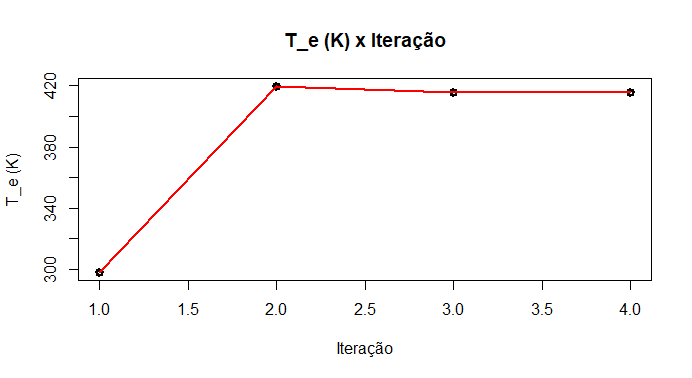
\includegraphics[scale=0.75]{Te_x_Iteracao_298K.png}
    \par{Fonte: elaboração própria.}
\end{figure}

\section{Análise e Discussão dos Resultados} \label{discussion}

A robustez da solução pode ser verificada alterando o valor do "chute" inicial. Para
valores iniciais de $T_e$ extremos de $T_{e_{inicial}} = 0 \un{K}$ e $T_{e_{inicial}} = 700 \un{K}$, obtemos 
temperaturas de equilíbrio respectivamente de $T_e = 415,95 \un{K}$ e $T_e = 415,96 \un{K}$,
comprovando que o valor de convergência do software não depende do chute inicial. 
As Figuras \ref*{fig:solucaoTe0e700} (a) e (b) exibem respectivamente a convergência para cada
valor extremos de $T_e$ inicial.

\begin{figure}[h!]
    \caption{\centering{Evolução da temperatura $T_e$ calculada pelo software a cada iteração do loop, para $T_e$ inicial
    (a) $0 \un{K}$ e (b) $700 \un{K}$.}}
    \label{fig:solucaoTe0e700}
    \centering
    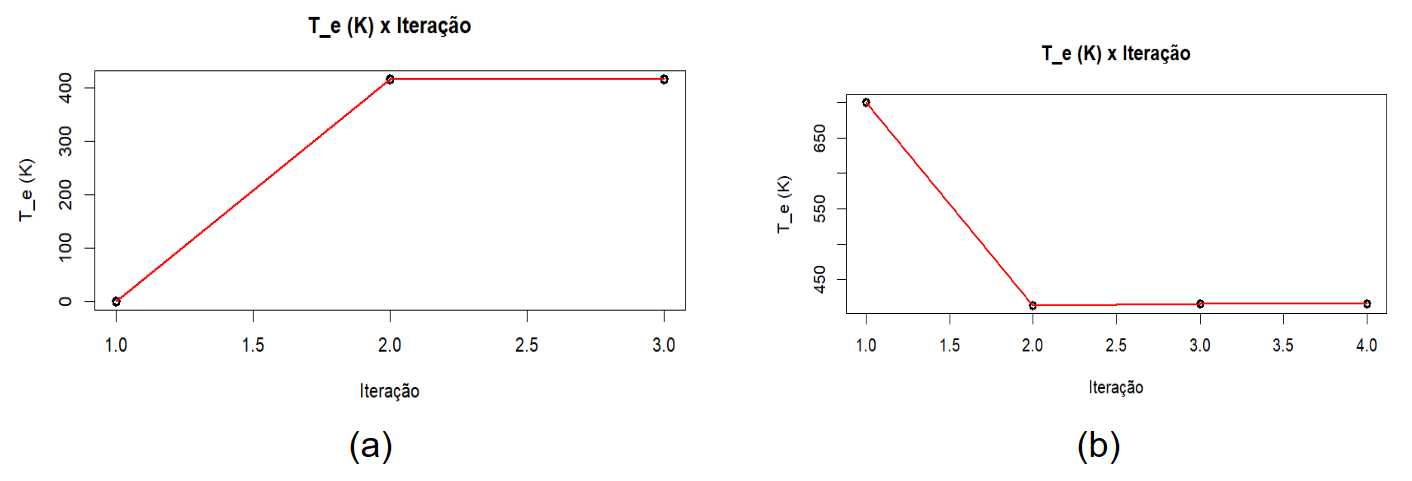
\includegraphics[scale=0.55]{Te_x_Iteracao_0e700K.png}
    \par{Fonte: elaboração própria.}
\end{figure}

Por fim, gostaríamos de elaborar um pouco mais sobre a decisão de considerar a convecção como natural, 
e não como forçada, apesar do ar sobre a placa possuir velocidade de $u_{\infty} = 10,8 \un{km/h}$. 
Se considerarmos a convecção como forçada, o regime de escoamento é determinado pelo Número de Reynolds
$Re$, e o valor do Número de Nusselt $Nu$ é dado por

\begin{equation}\label{eq:NuForced}
    Nu = \begin{cases}
        0,664 Re^{1/2}Pr^{1/3},  & Re \leq 5 \cdot 10^{5} \; \un{(Laminar}),                 \\
        \noalign{\vskip9pt}
        \left(0,037 Re^{4/5} - 871\right)Pr^{1/3},  & Re > 5 \cdot 10^{5} \; \un{(Turbulento)},                
    \end{cases}
\end{equation}

No código, a condição \eqref{eq:NuForced} pode ser feita através de 

\begin{lstlisting}
    if (Re < Re_critical) {
        # escoamento laminar
        Nu <- 0.664 * (Re)^(1/2) * (Pr)^(1/3)
      } else {
        # escoamento turbulento
        Nu <- (0.037 * Re^(4/5) - 871) * (Pr)^(1/3)
      }
\end{lstlisting}

No entanto, verificamos que, em condição de escoamento turbulento, o Número de Nusselts calculado era   
negativo devido à parcela $- 871$ da subtração, o que é claramente uma impossibilidade física.
Assim, optamos por considerar a convecção como natural para evitar essa inconsistência. \\

Para melhor estudar o comportamento da solução considerando-se a convecção como forçada, vamos considerar a velocidade do fluido $u_{\infty} = 30 \un{m/s}$, o que 
equivale a $u_{\infty} = 108 \un{km/h}$, que claramente é convecção forçada. Nesse caso, compilamos o software
novamente levando em consideração a condição \eqref{eq:NuForced}, obtendo os gráficos
da Figura \ref*{fig:solucaoTe50e700}.

\begin{figure}[h!]
    \caption{\centering{Evolução da temperatura $T_e$ calculada pelo software a cada iteração do loop, para $T_e$ inicial
    (a) $0 \un{K}$ e (b) $700 \un{K}$, com $u_{\infty} = 108 \un{km/h}$.}}
    \label{fig:solucaoTe50e700}
    \centering
    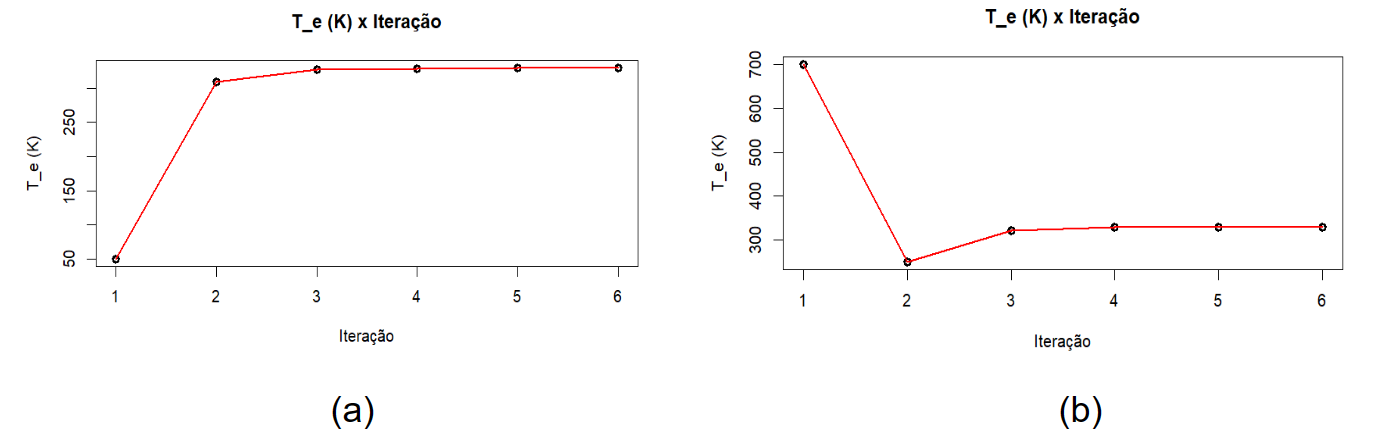
\includegraphics[scale=0.55]{Te_x_Iteracao_e700K_ui30.png}
    \par{Fonte: elaboração própria.}
\end{figure}

As soluções usando convecção forçada para altos valores de $u_{\infty}$ são robustas para vários valores 
inicias de $T_e$ "chutados", como mostra a Figura \ref*{fig:solucaoTe50e700}. Portanto, é válido considerar a convecção como natural para baixos
valores de $u_{\infty}$ e forçada para altos valores de $u_{\infty}$, uma vez que ambas convergem para a mesma 
temperatura de equilíbrio da face esquerda $T_e$ para diferentes valores iniciais estimados no código.

\section{Referências}

INCROPERA, Frank, et. al. Fundamentals of Heat and Mass Transfer. 6 ed. John Wilhey \& Sons Inc. 2007. \\

National Oceanic and Atmospheric Administation (NOAA). Estimating wind speed. Disponível em: https://www.weather.gov/pqr/wind.
Acesso em 22 de abr. de 2023.

\end{document}
